\documentclass{beamer}

\usepackage{tikz}
\usepackage{tikzlings}
\usepackage{tikzducks}

\definecolor{dblue}{RGB}{41,38,66}
\definecolor{dred}{RGB}{255,90,85}


\setbeamertemplate{background canvas}{
	\begin{tikzpicture}[remember picture, overlay]
	\node at (current page.center) {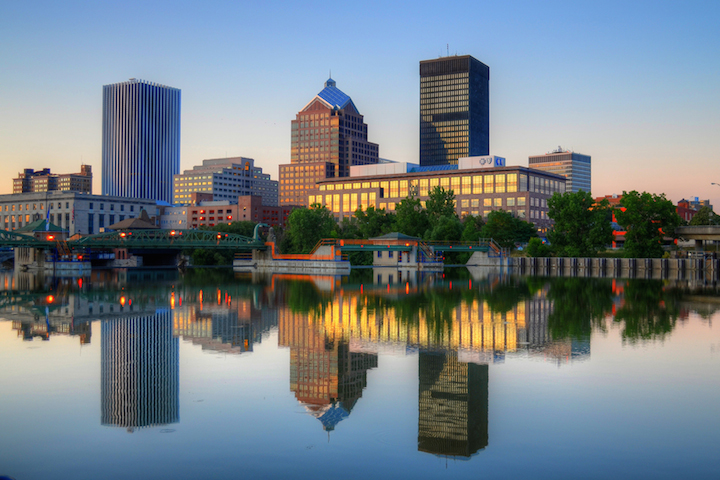
\includegraphics[height=1\paperheight]{Rochester}};
	\end{tikzpicture}
}
\setbeamertemplate{navigation symbols}{}
\usetikzlibrary {patterns.meta}
\tikzdeclarepattern{
  name=myStars,
  type=uncolored,
  bounding box={(-2pt,-2pt) and (2pt,2pt)},
  tile size={(\tikztilesize,\tikztilesize)},
  parameters={\tikzstarpoints,\tikzstarradius,\tikzstarrotate,\tikztilesize},
  tile transformation={rotate=\tikzstarrotate},
  defaults={
    points/.store in=\tikzstarpoints,points=5,
    radius/.store in=\tikzstarradius,radius=1pt,
    rotate/.store in=\tikzstarrotate,rotate=0,
    tile size/.store in=\tikztilesize,tile size=3pt,
}, code={
    \pgfmathparse{180/\tikzstarpoints}\let\a=\pgfmathresult
    \fill (90:\tikzstarradius) \foreach \i in {1,...,\tikzstarpoints}{
      -- (90+2*\i*\a-\a:\tikzstarradius/2) -- (90+2*\i*\a:\tikzstarradius)
    } -- cycle;
} }

\begin{document}
	
\begin{frame}<1->
	\begin{tikzpicture}[remember picture, overlay]
		\node[yshift=-0.65cm,inner sep=8pt,font=\Large\bfseries\color{white}] at (current page.north) {TUG'20 -- Rochester -- summer 2020};
		\begin{scope}[yshift=-3.25cm,xshift=7cm,scale=0.8]
			\duck[tshirt=dblue,cap=dred]
			\path[pattern=myStars,pattern color=white] \duckpathtshirt;
			\fill[dred] \duckpathjacket;	
			\stripes[rotate=95,color=white]
		\end{scope}
		\begin{scope}[yshift=-3.75cm,xshift=5cm,yscale=0.8,xscale=-0.8]
			\duck[tshirt=dblue,cap=white]
			\path[pattern=myStars,pattern color=white] \duckpathtshirt;
			\fill[dred] \duckpathjacket;	
			\stripes[rotate=95,color=white]
		\end{scope}		
		\begin{scope}[yshift=-4cm,xscale=-1,xshift=-2cm]
			\duck[tshirt=dblue,cap=dred]
			\path[pattern=myStars,pattern color=white] \duckpathtshirt;
			\fill[dred] \duckpathjacket;	
			\stripes[rotate=95,color=white]
		\end{scope}
		\begin{scope}[yshift=-5cm,xscale=1,xshift=9cm]
			\duck[tshirt=dblue,cap=dblue]
			\path[pattern=myStars,pattern color=white] \duckpathtshirt;
			\fill[dred] \duckpathjacket;	
			\stripes[rotate=95,color=white]
		\end{scope}

		\node[at=(current page.south),yshift=0.2cm,font=\tiny\color{white}]{Background: \url{https://commons.wikimedia.org/wiki/File:Downtown_Rochester,_NY_HDR_by_patrickashley.jpg}};
	\end{tikzpicture}
%	\pause[50]
\end{frame}	
	
\end{document}